%*----------- SLIDE -------------------------------------------------------------
\begin{frame}[t]{Fake News e Controle da Informação} 
    \begin{columns}[t]
        \column{.05\linewidth}
        \column{.65\linewidth}
        \begin{figure}
            %
\includegraphics[width=1\textwidth]{pista}
            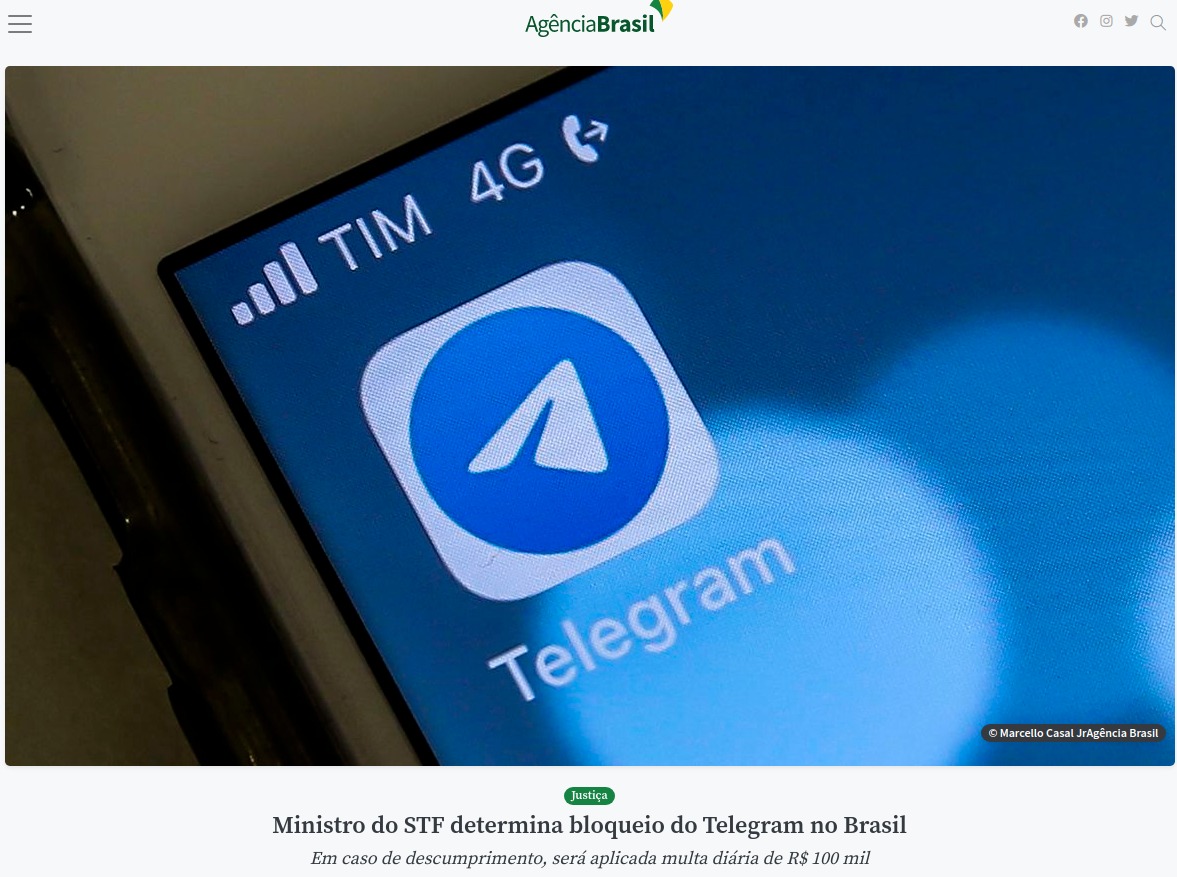
\includegraphics[width=0.73\textwidth]{liberdade/bloquio-telegram.png}
            \caption{\cite{bloqueiotelegram:online}}
        \end{figure}
        
        \column{.43\linewidth}
        \begin{center}
            \begin{figure}
                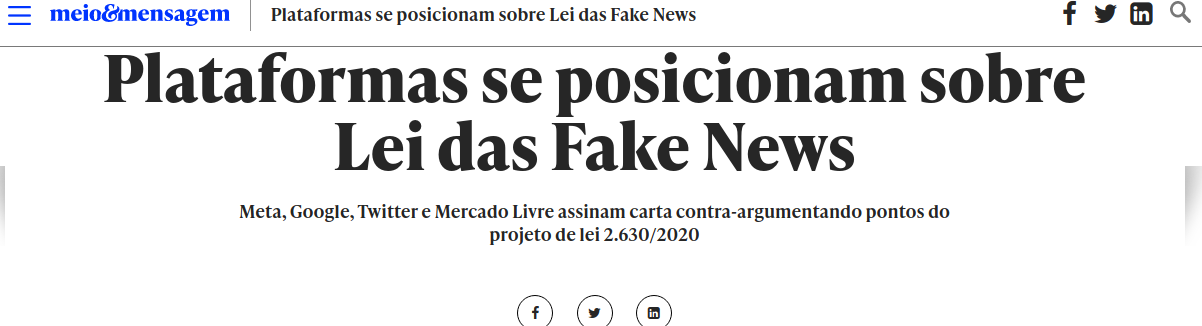
\includegraphics[width=0.6\textwidth]{liberdade/lei-fakenews-posicionamento.png}
                \caption{\cite{plataformasfakenews:online}}

                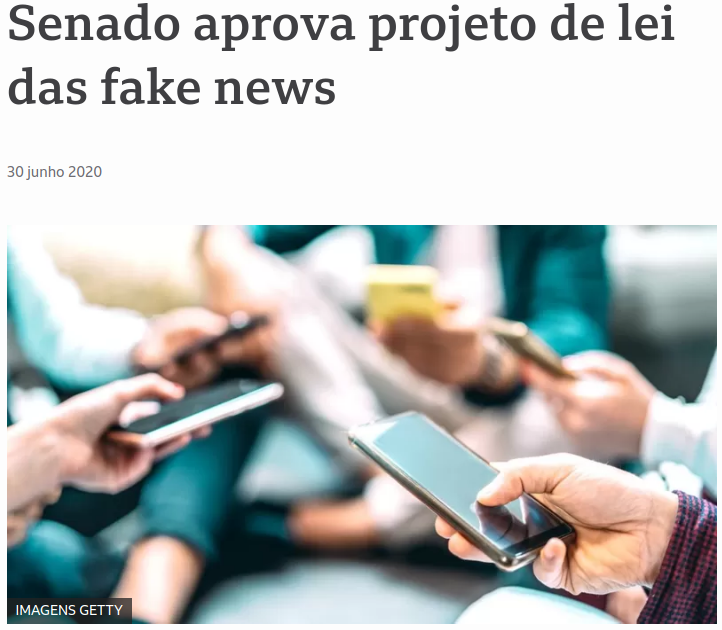
\includegraphics[width=0.55\textwidth]{liberdade/lei-fakenews.png}
                \caption{\cite{bbcfakenews:online}}
            \end{figure}
        \end{center}
    \end{columns}
%*----------- notes
    \note[item]{Notes can help you to remember important information. Turn on the notes option.}
\end{frame}

%*----------- SLIDE -------------------------------------------------------------
\begin{frame}[t]{Liberdade de Expressão} 
    "Estabelece normas relativas à transparência de redes sociais e de serviços de mensagens privadas, sobretudo no tocante à responsabilidade dos provedores pelo combate à desinformação e pelo aumento da transparência na internet, à transparência em relação a conteúdos patrocinados e à atuação do poder público, bem como estabelece sanções para o descumprimento da lei." \cite{fakenews-pl2630-2020}
    
    \vspace{0.25cm}
    "Posso não concordar com uma só palavra sua, mas defenderei até amorte  o  seu  direito  de  dizê-la" \cite{ribeiro2021ameacca}

    \vspace{0.25cm}
    "'Que é a verdade?' perguntou Pilatos (...)"
\end{frame}